% =====================================================================
% 옴니채널 프랜차이즈 매출 예측 시스템 — 요약 보고서
% Compiled with: xelatex bbq_summary.tex
% =====================================================================
\documentclass[11pt, a4paper]{article}

% --- Fonts & Language ---
\usepackage{fontspec}
\usepackage{xetexko}

% --- Page geometry ---
\usepackage[margin=2.3cm, top=2.8cm, bottom=2.8cm]{geometry}

% --- Packages ---
\usepackage{graphicx}
\usepackage{booktabs}
\usepackage{tabularx}
\usepackage{xcolor}
\usepackage{hyperref}
\usepackage{titlesec}
\usepackage{fancyhdr}
\usepackage{float}
\usepackage{enumitem}
\usepackage{colortbl}
\usepackage{tikz}
\usepackage{setspace}
\usepackage{ragged2e}
\usepackage{array}

% --- Font ---
\setmainfont{Apple SD Gothic Neo}

% --- Colors ---
\definecolor{darkblue}{HTML}{0F172A}
\definecolor{lightblue}{HTML}{D4E6F1}
\definecolor{accent}{HTML}{60A5FA}
\definecolor{red}{HTML}{DC2626}
\definecolor{gray}{HTML}{64748B}
\definecolor{kpibox}{HTML}{EBF5FB}
\definecolor{warnbox}{HTML}{FEF3C7}
\definecolor{greenbox}{HTML}{D1FAE5}
\definecolor{lightgray}{HTML}{F1F5F9}
\definecolor{bordergray}{HTML}{CBD5E1}
\definecolor{darkaccent}{HTML}{1E40AF}

% --- Hyperref ---
\hypersetup{
  colorlinks=true,
  linkcolor=darkaccent,
  urlcolor=accent,
  citecolor=darkblue,
  pdfborder={0 0 0}
}

% --- Section formatting ---
\titleformat{\section}
  {\Large\bfseries\color{darkblue}}
  {\thesection}{1em}{}
  [\vspace{-0.5em}\textcolor{accent}{\rule{\textwidth}{1.5pt}}]

\titleformat{\subsection}
  {\large\bfseries\color{darkblue}}
  {\thesubsection}{0.8em}{}

% --- Header / Footer ---
\pagestyle{fancy}
\fancyhf{}
\renewcommand{\headrulewidth}{0pt}
\fancyfoot[C]{\footnotesize\textcolor{gray}{한양대학교 경영대학 임보람 교수 연구실 \textperiodcentered{} 빅데이터 마케팅 연구그룹}}
\fancyfoot[R]{\footnotesize\textcolor{gray}{\thepage}}
\fancypagestyle{plain}{
  \fancyhf{}
  \renewcommand{\headrulewidth}{0pt}
  \fancyfoot[C]{\footnotesize\textcolor{gray}{한양대학교 경영대학 임보람 교수 연구실 \textperiodcentered{} 빅데이터 마케팅 연구그룹}}
  \fancyfoot[R]{\footnotesize\textcolor{gray}{\thepage}}
}

% --- Custom commands ---
\newcommand{\metriccard}[3]{%
  \begin{tikzpicture}
    \node[
      fill=kpibox,
      rounded corners=6pt,
      minimum width=4.8cm,
      minimum height=2.4cm,
      inner sep=8pt,
      align=center
    ] {
      {\small\textcolor{gray}{#1}}\\[3pt]
      {\LARGE\bfseries\textcolor{darkblue}{#2}}\\[2pt]
      {\footnotesize\textcolor{accent}{#3}}
    };
  \end{tikzpicture}%
}

\newcommand{\insightbox}[1]{%
  \vspace{0.5em}
  \noindent
  \fcolorbox{accent}{kpibox}{%
    \parbox{\dimexpr\textwidth-2\fboxsep-2\fboxrule}{%
      \vspace{0.4em}
      \textcolor{darkblue}{\textbf{핵심 인사이트}} \quad #1
      \vspace{0.4em}
    }%
  }%
  \vspace{0.5em}
}

\begin{document}

% =====================================================================
% COVER PAGE
% =====================================================================
\thispagestyle{empty}
\begin{tikzpicture}[remember picture, overlay]
  \fill[darkblue] (current page.north west) rectangle (current page.south east);
  \fill[accent] ([yshift=-9cm]current page.north west) rectangle ([yshift=-9.15cm]current page.north east);
  \fill[accent, opacity=0.3] ([yshift=3cm]current page.south west) rectangle ([yshift=3.08cm]current page.south east);
\end{tikzpicture}

\vspace*{4.5cm}

\begin{center}
  {\fontsize{30}{38}\selectfont\bfseries\textcolor{white}{옴니채널 프랜차이즈}}\\[0.4cm]
  {\fontsize{30}{38}\selectfont\bfseries\textcolor{white}{매출 예측 시스템}}\\[0.8cm]
  {\fontsize{18}{26}\selectfont\bfseries\textcolor{accent}{채널별 성과 동인 분석 및 AI 기반 수요 예측}}\\[1.5cm]
  \textcolor{accent}{\rule{8cm}{0.8pt}}\\[1.5cm]
  {\fontsize{13}{18}\selectfont\textcolor{lightblue}{국내 대형 치킨 프랜차이즈 349개 매장 실증 분석}}\\[0.3cm]
  {\fontsize{13}{18}\selectfont\textcolor{lightblue}{배달 \textperiodcentered{} 매장식사 채널별 매출 예측 모델}}\\[2.5cm]
  {\fontsize{12}{16}\selectfont\textcolor{white}{한양대학교 경영대학}}\\[0.3cm]
  {\fontsize{13}{18}\selectfont\bfseries\textcolor{accent}{임보람 교수 연구실}}\\[0.3cm]
  {\fontsize{11}{15}\selectfont\textcolor{lightblue}{빅데이터 마케팅 연구그룹}}\\[2cm]
  {\footnotesize\textcolor{gray}{Summary Report \textperiodcentered{} JRCS 게재}}
\end{center}

\newpage

% =====================================================================
% PAGE 2: EXECUTIVE SUMMARY
% =====================================================================
\section*{Executive Summary}

\vspace{0.5em}

매장식사 채널 R\textsuperscript{2} 0.986(96\%), 배달 채널 R\textsuperscript{2} 0.948 --- 국내 대형 치킨 프랜차이즈 \textbf{349개 매장}의 채널별 매출을 거의 완벽하게 예측하는 AI 모델을 개발했다. 총 \textbf{224개 모델}을 체계적으로 비교 분석하여, 채널별 최적 예측 전략을 도출했다.

\vspace{1em}

\begin{center}
\metriccard{매장식사 R\textsuperscript{2}}{0.986}{예측 정확도 96\%}
\hfill
\metriccard{배달 R\textsuperscript{2}}{0.948}{배달 채널 예측}
\hfill
\metriccard{분석 규모}{349 매장}{224개 모델 비교}
\end{center}

\vspace{1em}

\insightbox{프랜차이즈 매출의 핵심 동인은 인구통계(상권 특성)이며, 이는 배달과 매장식사 \textbf{모든 채널에서 공통적}으로 가장 중요한 예측 변수이다. 리뷰 데이터를 결합하면 예측 성능이 추가로 향상된다.}

\vspace{0.5em}

\noindent\textcolor{gray}{\small 본 연구는 \textit{Journal of Retailing and Consumer Services} (JRCS)에 게재되었습니다.}

\newpage

% =====================================================================
% PAGE 3: 채널별 예측 성능
% =====================================================================
\section*{채널별 예측 성능}

\vspace{0.5em}

224개 모델을 체계적으로 비교한 결과, 매장식사와 배달 채널 모두에서 90\% 이상의 높은 예측 정확도를 달성했다. 특히 매장식사 채널은 R\textsuperscript{2} 0.986으로 거의 완벽한 수준이다.

\vspace{1em}

\begin{figure}[H]
  \centering
  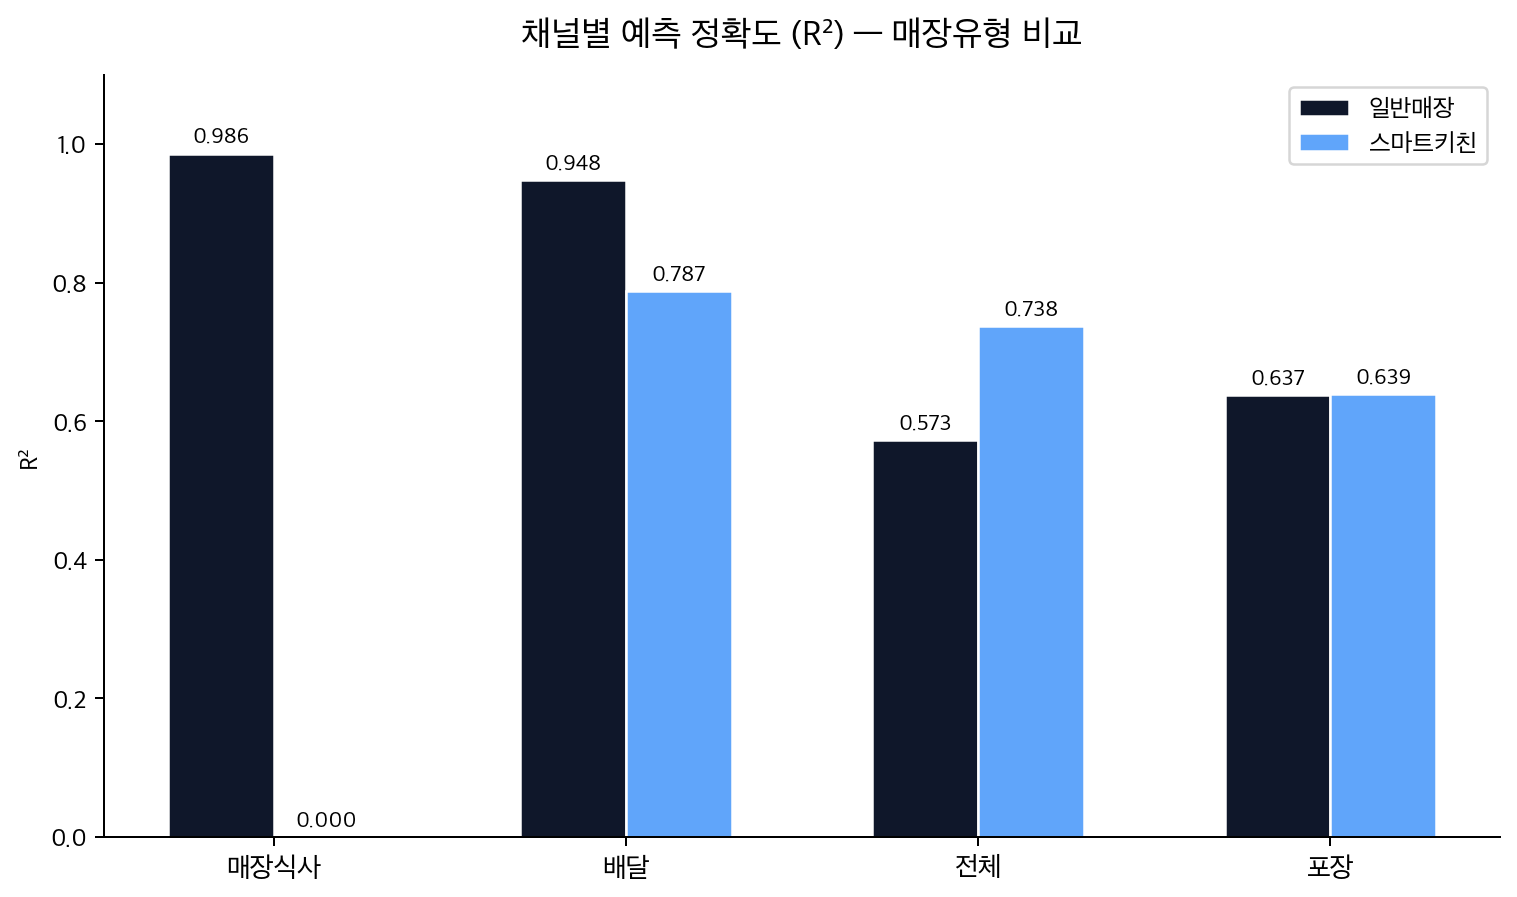
\includegraphics[width=0.92\textwidth]{bbq_channel_r2.png}
  \caption{채널별 예측 모델 성능 비교}
\end{figure}

\vspace{0.5em}

\insightbox{채널별로 매출 동인이 다르기 때문에, 각 채널에 최적화된 예측 모델이 필요하다. 단일 통합 모델 대비 채널별 모델이 일관되게 우수한 성능을 보인다.}

\newpage

% =====================================================================
% PAGE 4: 핵심 발견 — 리뷰 및 입지
% =====================================================================
\section*{핵심 발견: 인구통계와 리뷰의 역할}

\vspace{0.5em}

인구통계(상권 특성)는 모든 채널에서 가장 중요한 매출 예측 변수이다. 여기에 리뷰 데이터를 결합하면 예측 성능이 추가로 향상되며, 이는 \textbf{고객 피드백이 매출에 직접적으로 영향}을 미침을 보여준다.

\vspace{1em}

\begin{figure}[H]
  \centering
  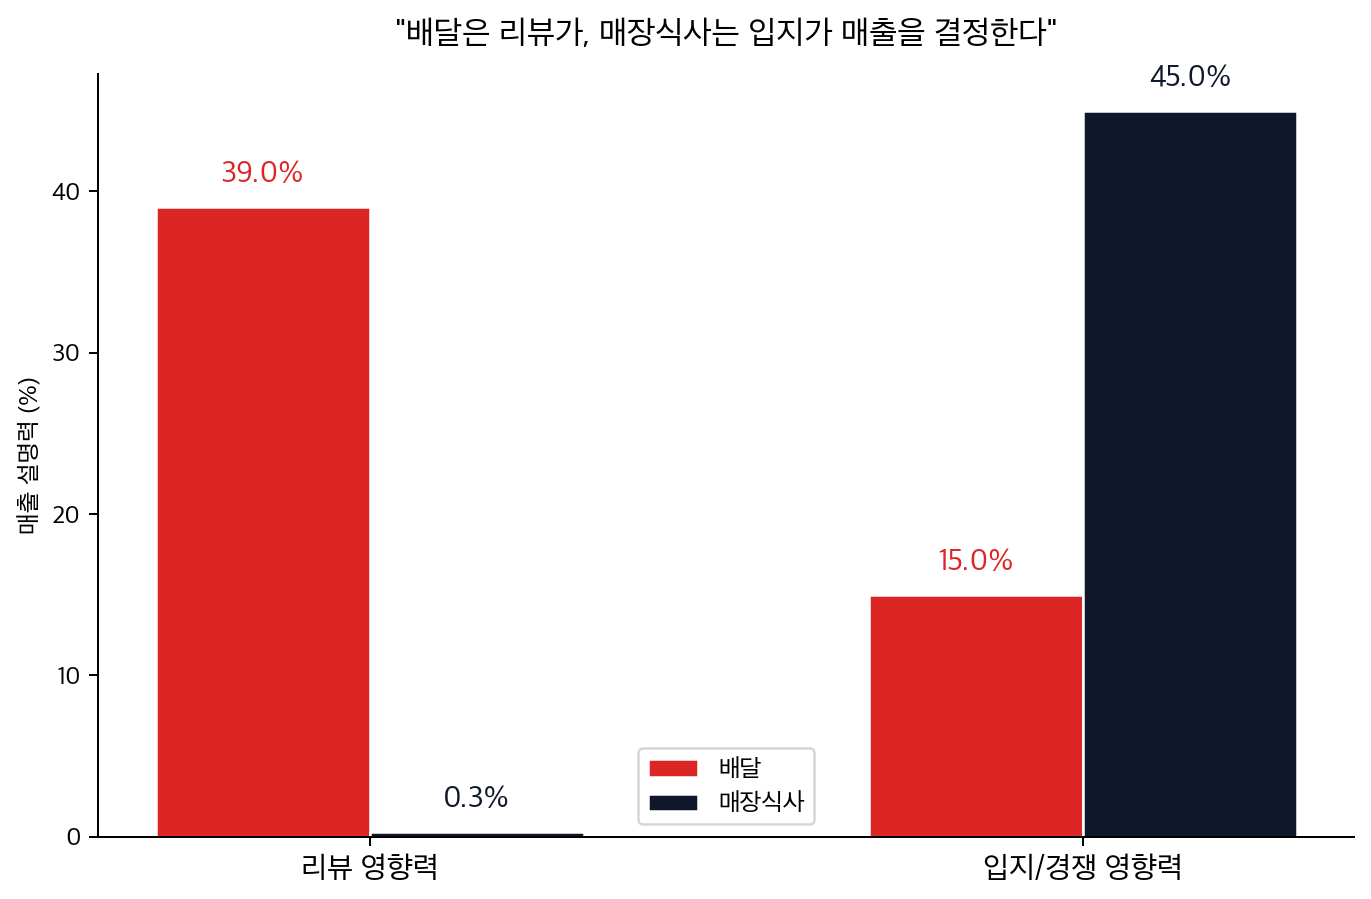
\includegraphics[width=0.92\textwidth]{bbq_review_vs_location.png}
  \caption{리뷰 데이터와 입지 특성의 매출 예측 기여도}
\end{figure}

\vspace{1em}

\begin{figure}[H]
  \centering
  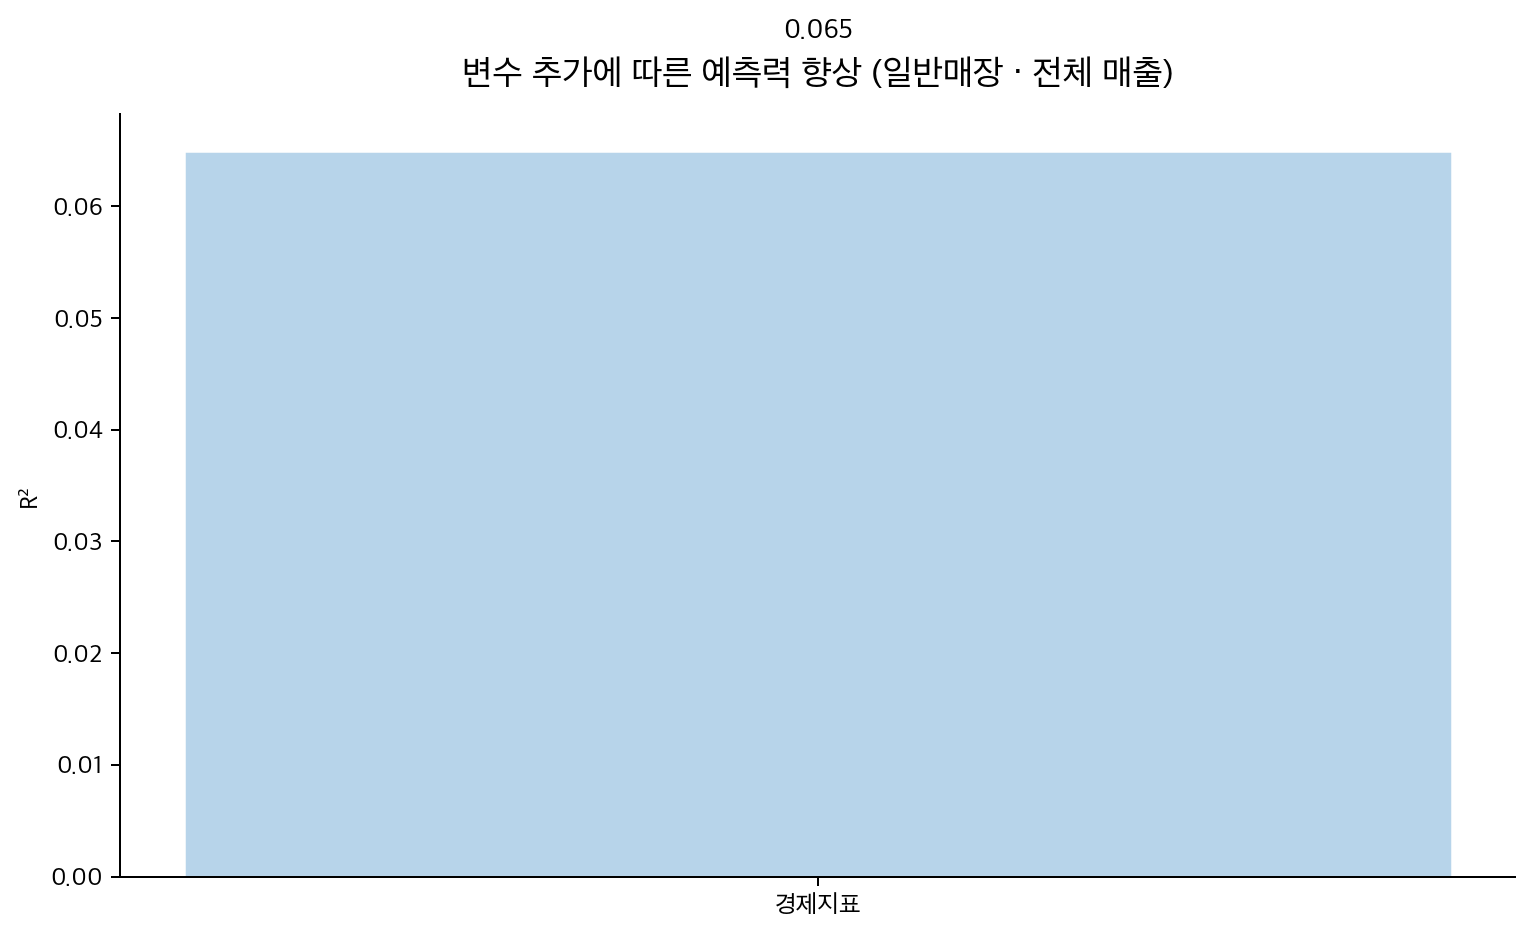
\includegraphics[width=0.92\textwidth]{bbq_feature_improvement.png}
  \caption{변수 추가에 따른 예측 성능 향상}
\end{figure}

\newpage

% =====================================================================
% PAGE 5: 전략적 시사점 + 문의
% =====================================================================
\section*{전략적 시사점}

\vspace{0.5em}

\noindent
\fcolorbox{bordergray}{lightgray}{%
  \parbox{\dimexpr\textwidth-2\fboxsep-2\fboxrule}{%
    \vspace{0.8em}
    {\large\bfseries\textcolor{darkblue}{1. 데이터 기반 출점 전략}}\\[6pt]
    {\normalsize 인구통계가 매출의 핵심 동인이므로, 상권 분석 데이터를 활용한 출점 의사결정이 매출 극대화의 핵심이다. R\textsuperscript{2} 0.986 수준의 예측 모델로 신규 매장 매출을 사전에 추정할 수 있다.}
    \vspace{0.6em}
  }%
}

\vspace{0.8em}

\noindent
\fcolorbox{bordergray}{lightgray}{%
  \parbox{\dimexpr\textwidth-2\fboxsep-2\fboxrule}{%
    \vspace{0.8em}
    {\large\bfseries\textcolor{darkblue}{2. 리뷰 관리의 매출 효과 실증}}\\[6pt]
    {\normalsize 리뷰 데이터가 매출 예측 성능을 유의미하게 향상시킨다는 실증 결과는, 리뷰 관리가 단순 CS가 아닌 매출 성장 전략임을 보여준다.}
    \vspace{0.6em}
  }%
}

\vspace{0.8em}

\noindent
\fcolorbox{bordergray}{lightgray}{%
  \parbox{\dimexpr\textwidth-2\fboxsep-2\fboxrule}{%
    \vspace{0.8em}
    {\large\bfseries\textcolor{darkblue}{3. 채널별 차별화 전략 수립}}\\[6pt]
    {\normalsize 배달과 매장식사 채널은 매출 동인이 다르므로, 각 채널에 맞는 차별화된 마케팅 및 운영 전략이 필요하다.}
    \vspace{0.6em}
  }%
}

\vspace{3em}

\begin{center}
\fcolorbox{darkaccent}{lightblue}{%
  \parbox{0.85\textwidth}{%
    \vspace{1em}
    \begin{center}
    {\Large\bfseries\textcolor{darkblue}{전체 보고서 및 상세 분석은}}\\[8pt]
    {\Large\bfseries\textcolor{darkblue}{연구실로 문의해주세요}}\\[12pt]
    {\normalsize\textcolor{gray}{한양대학교 경영대학 임보람 교수 연구실}}\\[4pt]
    {\normalsize\textcolor{gray}{빅데이터 마케팅 연구그룹}}
    \end{center}
    \vspace{1em}
  }%
}
\end{center}

\end{document}
